%%%%%%%%%%%%%%%%%%%%%%%%%%%%%%%%%%%%%%%%%
% Short Sectioned Assignment LaTeX Template Version 1.0 (5/5/12)
% This template has been downloaded from: http://www.LaTeXTemplates.com
% Original author:  Frits Wenneker (http://www.howtotex.com)
% License: CC BY-NC-SA 3.0 (http://creativecommons.org/licenses/by-nc-sa/3.0/)
%%%%%%%%%%%%%%%%%%%%%%%%%%%%%%%%%%%%%%%%%

%----------------------------------------------------------------------------------------
%	PACKAGES AND OTHER DOCUMENT CONFIGURATIONS
%----------------------------------------------------------------------------------------

\documentclass[paper=a4, fontsize=11pt]{scrartcl} % A4 paper and 11pt font size

% ---- Entrada y salida de texto -----

\usepackage[T1]{fontenc} % Use 8-bit encoding that has 256 glyphs
\usepackage[utf8]{inputenc}
%\usepackage{fourier} % Use the Adobe Utopia font for the document - comment this line to return to the LaTeX default

% ---- Idioma --------

\usepackage[spanish, es-tabla]{babel} % Selecciona el español para palabras introducidas automáticamente, p.ej. "septiembre" en la fecha y especifica que se use la palabra Tabla en vez de Cuadro

\usepackage{eurosym}
\usepackage{enumitem}

% ---- Otros paquetes ----

\usepackage{url} % ,href} %para incluir URLs e hipervínculos dentro del texto (aunque hay que instalar href)
\usepackage{amsmath,amsfonts,amsthm} % Math packages
%\usepackage{graphics,graphicx, floatrow} %para incluir imágenes y notas en las imágenes
\usepackage{graphics,graphicx, float} %para incluir imágenes y colocarlas

% Para hacer tablas comlejas
%\usepackage{multirow}
%\usepackage{threeparttable}

%\usepackage{sectsty} % Allows customizing section commands
%\allsectionsfont{\centering \normalfont\scshape} % Make all sections centered, the default font and small caps

\usepackage{fancyhdr} % Custom headers and footers
\pagestyle{fancyplain} % Makes all pages in the document conform to the custom headers and footers
\fancyhead{} % No page header - if you want one, create it in the same way as the footers below
\fancyfoot[L]{} % Empty left footer
\fancyfoot[C]{} % Empty center footer
\fancyfoot[R]{\thepage} % Page numbering for right footer
\renewcommand{\headrulewidth}{0pt} % Remove header underlines
\renewcommand{\footrulewidth}{0pt} % Remove footer underlines
\setlength{\headheight}{13.6pt} % Customize the height of the header

\numberwithin{equation}{section} % Number equations within sections (i.e. 1.1, 1.2, 2.1, 2.2 instead of 1, 2, 3, 4)
\numberwithin{figure}{section} % Number figures within sections (i.e. 1.1, 1.2, 2.1, 2.2 instead of 1, 2, 3, 4)
\numberwithin{table}{section} % Number tables within sections (i.e. 1.1, 1.2, 2.1, 2.2 instead of 1, 2, 3, 4)

\setlength\parindent{0pt} % Removes all indentation from paragraphs - comment this line for an assignment with lots of text

\newcommand{\horrule}[1]{\rule{\linewidth}{#1}} % Create horizontal rule command with 1 argument of height


%----------------------------------------------------------------------------------------
%	TÍTULO Y DATOS DEL ALUMNO
%----------------------------------------------------------------------------------------

\title{	
\normalfont \normalsize 
\textsc{\textbf{Ingeniería de Servidores (2016-2017)} \\ Grado en Ingeniería Informática \\ Universidad de Granada} \\ [25pt] % Your university, school and/or department name(s)
\horrule{0.5pt} \\[0.4cm] % Thin top horizontal rule
\huge Memoria Práctica 5 \\ % The assignment title
\horrule{2pt} \\[0.5cm] % Thick bottom horizontal rule
}

\author{Cristian Vélez Ruiz} % Nombre y apellidos

\date{\normalsize\today} % Incluye la fecha actual

%----------------------------------------------------------------------------------------
% DOCUMENTO
%----------------------------------------------------------------------------------------
\begin{document}

\maketitle % Muestra el Título

\newpage %inserta un salto de página

\tableofcontents % para generar el índice de contenidos

\listoffigures

\listoftables

\newpage

%----------------------------------------------------------------------------------------
%	Cuestión 1
%----------------------------------------------------------------------------------------
\section[Cuestión 1]{Al modificar los valores del kernel de este modo, no logramos que persistan después de reiniciar la máquina. ¿Qué archivo hay que editar para que los cambios sean permanentes?}

Para que los cambios que realicemos con sysctl sean persistentes necesitamos modificar el archivo \textbf{/etc/sysctl.conf}, donde se guarda la configuración del kernel y se cargará una vez arrancado nuestro sistema.

En mi caso modificare la variable para que cuando haya un kernel panic se reinicie a los 10 segundos.

\begin{itemize}
	\item Observamos el estado actual de la variable con \textit{sysctl -a | grep panic}:
	
	\begin{figure}[H] %con el [H] le obligamos a situar aquí la figura
		\centering
		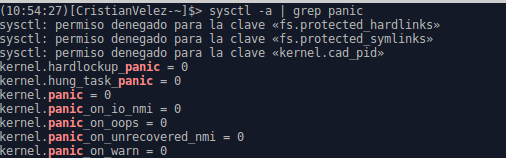
\includegraphics[scale=0.5]{pics/kernel}  %el parámetro scale permite agrandar o achicar la imagen. En el nombre de archivo puede especificar directorios
		\caption{Estado kernel panic} \label{fig:kernel1}
	\end{figure}
	Como se puede apreciar esta configurado a 0.
	
	\item Ahora para cambiarlo a 10 debemos hacer \textit{sudo sysctl -w kernel.panic=10}.
	
	\begin{figure}[H] %con el [H] le obligamos a situar aquí la figura
		\centering
		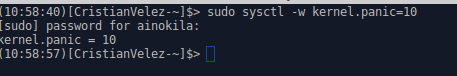
\includegraphics[scale=0.5]{pics/kernel1}  %el parámetro scale permite agrandar o achicar la imagen. En el nombre de archivo puede especificar directorios
		\caption{Cambiando kernel panic} \label{fig:kernel2}
	\end{figure}

	\item Una vez modificado debemos hacerlo persistente añadiendo al archivo \textbf{/etc/sysctl.conf} con \textbf{echo "kernel.panic = 10" >> /etc/sysctl.conf}.

\item Una vez realizado actualizamos la configuracion de sysctl con \textit{sysctl -p}.

\begin{figure}[H] %con el [H] le obligamos a situar aquí la figura
	\centering
	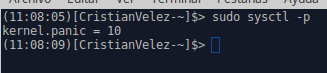
\includegraphics[scale=0.5]{pics/kernel2}  %el parámetro scale permite agrandar o achicar la imagen. En el nombre de archivo puede especificar directorios
	\caption{Cambiando kernel panic} \label{fig:kernel3}
\end{figure}

Como se puede apreciar se ha actualizado kernel.panic y ya es permanente.
\end{itemize}


	
	

%----------------------------------------------------------------------------------------
%	Cuestión 2
%----------------------------------------------------------------------------------------
\section[Cuestión 2]{¿Con qué opción se muestran todos los parámetros modificables en tiempo de ejecución? Elija dos parámetros y explique, en dos líneas, qué función tienen.}

Para mostrar los parametros en tiempo de ejecución se usa \textbf{sysctl -a} \cite{kernel}

\begin{figure}[H] %con el [H] le obligamos a situar aquí la figura
	\centering
	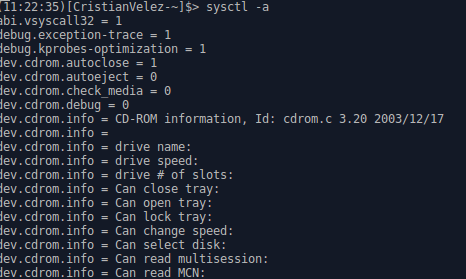
\includegraphics[scale=0.5]{pics/a}  %el parámetro scale permite agrandar o achicar la imagen. En el nombre de archivo puede especificar directorios
	\caption{sysctl -a} \label{fig:kernel4}
\end{figure}

\begin{itemize}
	\item \textbf{kernel.panic\_on\_stackoverflow} : Si se produce un desbordamiento de pila y esta configurado a 0, intentara continuar con la operacion , en cambio si esta a 1 entrara en modo panico.
	
	\item \textbf{kernel.pid\_max} :Cuando el siguiente PID del kernel alcanza este valor, se ajusta a un valor mínimo de PID, ni el minimo ni el maximo se utilizan.
\end{itemize}


%----------------------------------------------------------------------------------------
%	Cuestión 3
%----------------------------------------------------------------------------------------
\section[Cuestión 3]{a) Realice una copia de seguridad del registro y restáurela, ilustre el proceso con capturas. b) Abra una ventana mostrando el editor del	registro.}

Para realizar la copia debemos ir a regedit (editor de registros):

\begin{figure}[H] %con el [H] le obligamos a situar aquí la figura
	\centering
	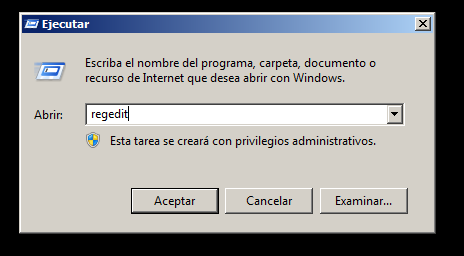
\includegraphics[scale=0.5]{pics/reg}  %el parámetro scale permite agrandar o achicar la imagen. En el nombre de archivo puede especificar directorios
	\caption{Copia seguridad regedit} \label{fig:reg}
\end{figure}

Una vez abierto damos a exportar:

\begin{figure}[H] %con el [H] le obligamos a situar aquí la figura
	\centering
	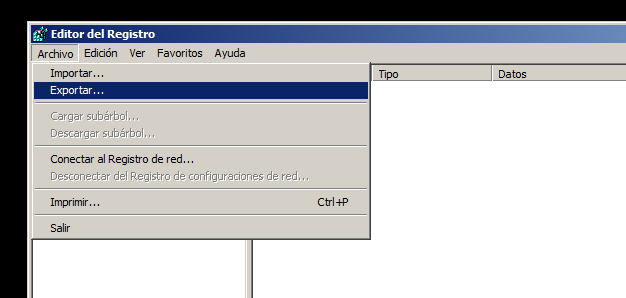
\includegraphics[scale=0.5]{pics/reg1}  %el parámetro scale permite agrandar o achicar la imagen. En el nombre de archivo puede especificar directorios
	\caption{Copia seguridad regedit 1} \label{fig:reg1}
\end{figure}

Añadimos el nombre a la copia de seguridad y donde queremos guardarla:

Una vez abierto damos a exportar:

\begin{figure}[H] %con el [H] le obligamos a situar aquí la figura
	\centering
	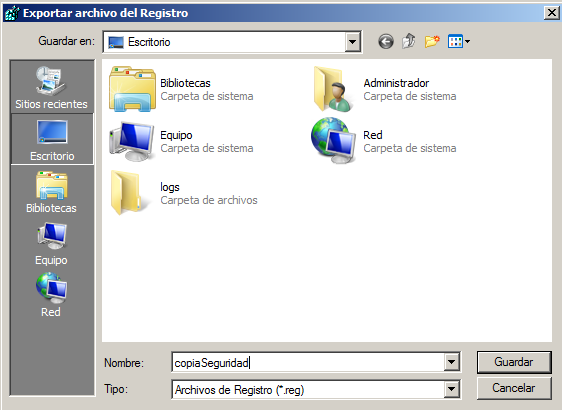
\includegraphics[scale=0.5]{pics/red2}  %el parámetro scale permite agrandar o achicar la imagen. En el nombre de archivo puede especificar directorios
	\caption{Copia seguridad regedit 2} \label{fig:reg2}
\end{figure}

Ya tenemos nuestra copia de seguridad realizada.

\begin{figure}[H] %con el [H] le obligamos a situar aquí la figura
	\centering
	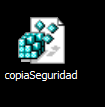
\includegraphics[scale=0.5]{pics/reg3}  %el parámetro scale permite agrandar o achicar la imagen. En el nombre de archivo puede especificar directorios
	\caption{Copia seguridad regedit 3} \label{fig:reg3}
\end{figure}

Para hacer el paso contrario, restarurar la copia de seguridad, vamos a importar:

\begin{figure}[H] %con el [H] le obligamos a situar aquí la figura
	\centering
	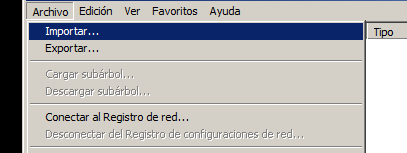
\includegraphics[scale=0.5]{pics/reg4}  %el parámetro scale permite agrandar o achicar la imagen. En el nombre de archivo puede especificar directorios
	\caption{Copia seguridad regedit 4} \label{fig:reg4}
\end{figure}

Seleccionamos la copia de seguridad a restaurar:

\begin{figure}[H] %con el [H] le obligamos a situar aquí la figura
	\centering
	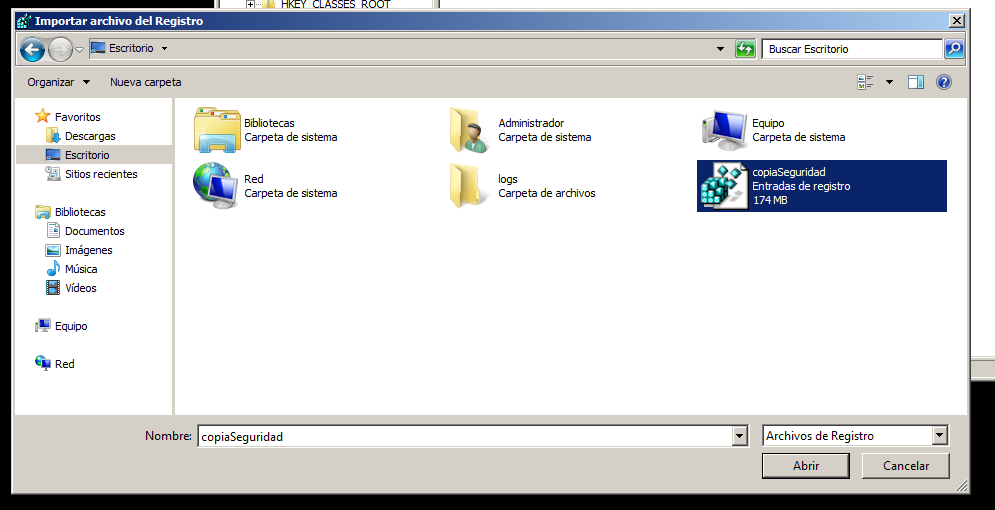
\includegraphics[scale=0.5]{pics/reg5}  %el parámetro scale permite agrandar o achicar la imagen. En el nombre de archivo puede especificar directorios
	\caption{Copia seguridad regedit 5} \label{fig:reg5}
\end{figure}

Seleccionamos abrir y comenzará el proceso de restauracion.

\begin{figure}[H] %con el [H] le obligamos a situar aquí la figura
	\centering
	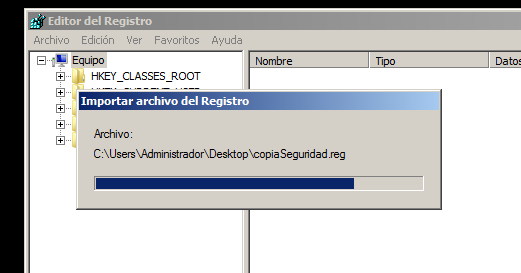
\includegraphics[scale=0.5]{pics/reg6}  %el parámetro scale permite agrandar o achicar la imagen. En el nombre de archivo puede especificar directorios
	\caption{Copia seguridad regedit 6} \label{fig:reg6}
\end{figure}

Una vez finalice ya tenemos restaurada la copia de seguridad.



%----------------------------------------------------------------------------------------
%	Cuestión 4
%----------------------------------------------------------------------------------------
\section[Cuestión 4]{ Enumere qué elementos se pueden configurar en Apache y en IIS para que Moodle funcione mejor.}

En Apache algunos de los elementos que podemos configurar son:

\begin{itemize}
	\item MaxClients para evitar que el sistema se quede sin memoria.
	\item Reducir el numero de modulos que Apache carga desde httpd.conf para reducir el uso de memoria.
	\item Disminuir MaxRequestsPerChild a 20-30.
	\item Cnfigurar un Reverse Proxy server para reducir la carga del servidor para la descarga de archivos con imagenes.
	\item Configurar el Directory Index DirectoryIndex correctamente para evitar la negociación de contenido.
	\item Desactivar HostnameLookups para reducir la latencia del dns.
	\item Reducir el TimeOut a 30-60.
	
\end{itemize}

En ISS algunos de los elementos que podemos configurar son:

\begin{itemize}
	\item ListenBackLog es el equivalente de KeepAliveTimeout establecer entre 2-5.
	\item MemCacheSize tamaño de la memoria cache, por defecto esta configurado a la mitad disponible.
	\item ObjectCacheTTL tiempo en el que los objetos permanecen en la memoria cache.
	
	
\end{itemize}

%----------------------------------------------------------------------------------------
%	Cuestión 5
%----------------------------------------------------------------------------------------
\section[Cuestión 5]{ Ajuste la compresión en el servidor y analice su comportamiento usando varios valores para el tamaño de archivo a partir del cual comprimir. Para comprobar que está comprimiendo puede usar el navegador o comandos como curl (see url) o lynx. Muestre capturas de pantalla de todo el proceso}

Para poder comprobar la compresión del servidor voy a modificar la pagina por defecto del servidor como hicimos en la practica anterior casi 2KiB.

\begin{figure}[H] %con el [H] le obligamos a situar aquí la figura
	\centering
	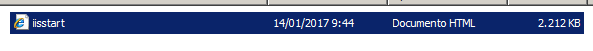
\includegraphics[scale=0.5]{pics/2}  %el parámetro scale permite agrandar o achicar la imagen. En el nombre de archivo puede especificar directorios
	\caption{Archivo por defecto} \label{fig:1}
\end{figure}

Una vez realizado vamos a la configuración de IIS y después al apartado Compresión y habilitamos las pestañas de compresión estática, y también configuramos sus parámetros.

\begin{figure}[H] %con el [H] le obligamos a situar aquí la figura
	\centering
	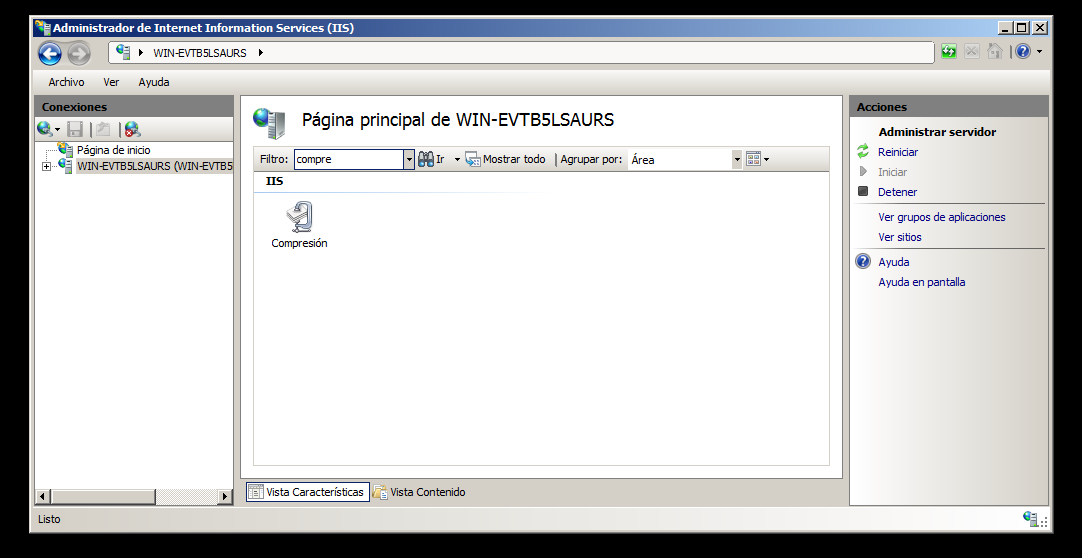
\includegraphics[scale=0.5]{pics/1}  %el parámetro scale permite agrandar o achicar la imagen. En el nombre de archivo puede especificar directorios
	\caption{Compresión del servidor} \label{fig:2}
\end{figure}

\begin{figure}[H] %con el [H] le obligamos a situar aquí la figura
	\centering
	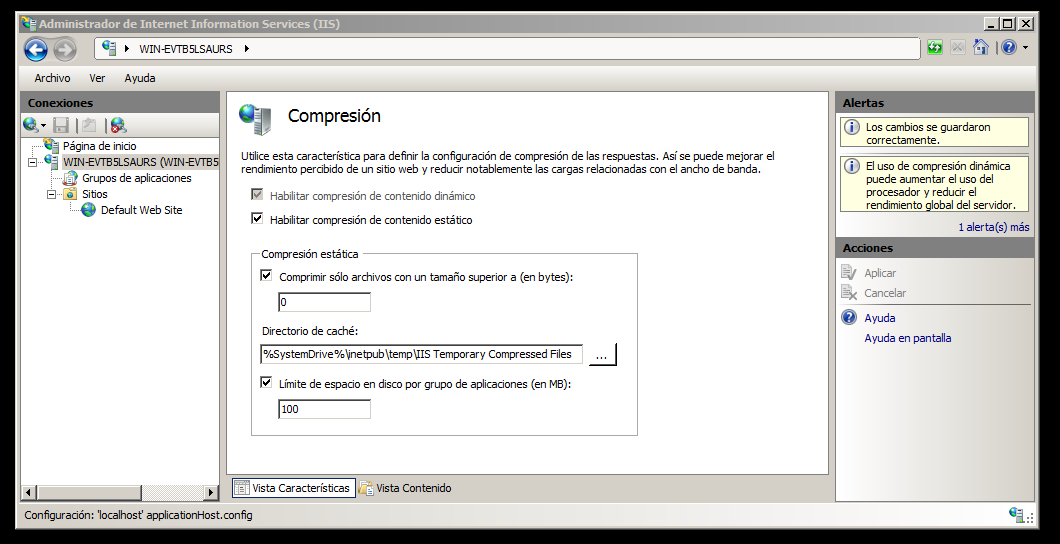
\includegraphics[scale=0.5]{pics/3}  %el parámetro scale permite agrandar o achicar la imagen. En el nombre de archivo puede especificar directorios
	\caption{Compresión del servidor 2} \label{fig:3}
\end{figure}

Desde otra maquina lanzaré la orden \textit{curl -I -H 'Accept-Encoding:gzip,deflate'} antes de aplicar los cambios y una vez aplicados para ver el tamaño de la  respuesta a la petición.

\begin{figure}[H] %con el [H] le obligamos a situar aquí la figura
	\centering
	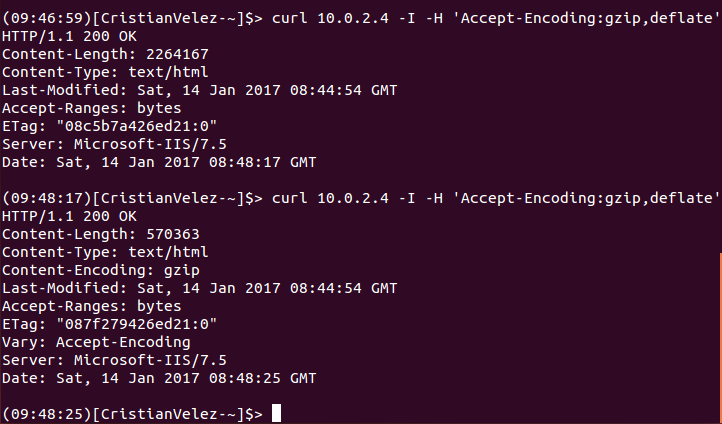
\includegraphics[scale=0.5]{pics/4}  %el parámetro scale permite agrandar o achicar la imagen. En el nombre de archivo puede especificar directorios
	\caption{Compresión del servidor 3} \label{fig:4}
\end{figure}

Como se puede apreciar la longitud de la respuesta ha pasado de 2264167 a 570363, lo que es casi un cuarto de su longitud anterior.



%----------------------------------------------------------------------------------------
%	Cuestión 6
%----------------------------------------------------------------------------------------
\section[Cuestión 6]{Usted parte de un SO con ciertos parámetros definidos en la	instalación (Práctica 1), ya sabe instalar servicios (Práctica 2) y cómo monitorizarlos (Práctica 3) cuando los somete a cargas (Práctica 4). Al igual que ha visto cómo se puede mejorar un servidor web (Práctica 5 Sección 3.1), elija un servicio (el que usted quiera) y modifique un parámetro para	mejorar su comportamiento. 6.b) Monitorice el servicio antes y después de la modificación del parámetro aplicando cargas al sistema (antes y después) mostrando los resultados de la monitorización.}

\begin{enumerate}[label=(\alph*)]
	\item 
Modificaré el servicio apache dos parametros:

\begin{itemize}
	\item MaxKeepAliveRequest: Número máximo de peticiones a permitir en una conexión persistente. Antes estaba: 100 , ahora: 64
	
	\item KeepAliveTimeout: Número de segundos a esperar a la siguiente petición de algún cliente. Antes estaba: 5 , ahora: 3
\end{itemize}

Antes de que sea modificado se hará la prueba del ejercicio 6.b.\\

Para modificar estos datos debemos ir a /etc/apache2/apache2.conf, hacemos una copia de seguridad, seguidamente editamos los valores y reiniciamos el servicio.

\begin{figure}[H] %con el [H] le obligamos a situar aquí la figura
	\centering
	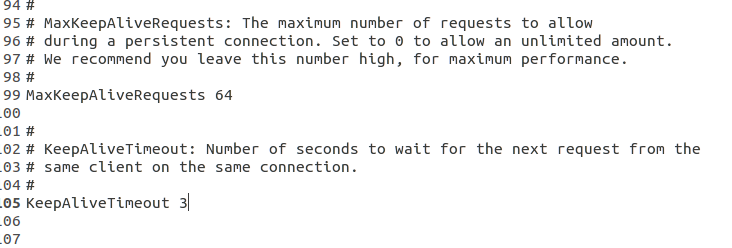
\includegraphics[scale=0.5]{pics/12}  %el parámetro scale permite agrandar o achicar la imagen. En el nombre de archivo puede especificar directorios
	\caption{Optimizando Apache} \label{fig:5}
\end{figure}

\begin{figure}[H] %con el [H] le obligamos a situar aquí la figura
	\centering
	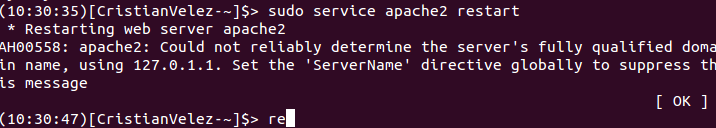
\includegraphics[scale=0.5]{pics/13}  %el parámetro scale permite agrandar o achicar la imagen. En el nombre de archivo puede especificar directorios
	\caption{Optimizando Apache 1} \label{fig:6}
\end{figure}

\item Para obtener  monitorizar el rendimiento usaré Apache Benchmark como en la práctica anterior con ab -n 50000 -c 50 http://direccion/index.html, antes y después de la modificación.

\begin{itemize}
	\item \textbf{Configuración por defecto:}
	
	\begin{figure}[H] %con el [H] le obligamos a situar aquí la figura
		\centering
		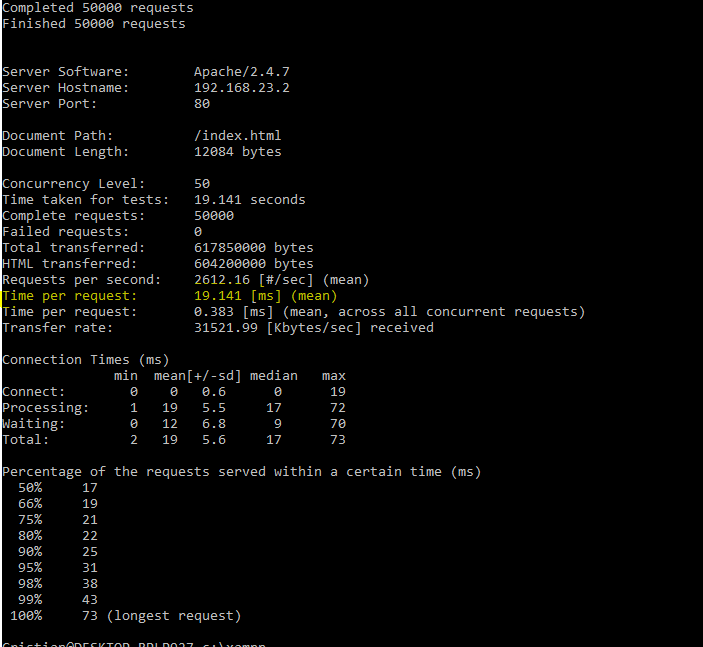
\includegraphics[scale=0.5]{pics/111}  %el parámetro scale permite agrandar o achicar la imagen. En el nombre de archivo puede especificar directorios
		\caption{Configuración por defecto} \label{fig:7}
	\end{figure}
	
	\item \textbf{Configuración modificada:}
	
		\begin{figure}[H] %con el [H] le obligamos a situar aquí la figura
		\centering
		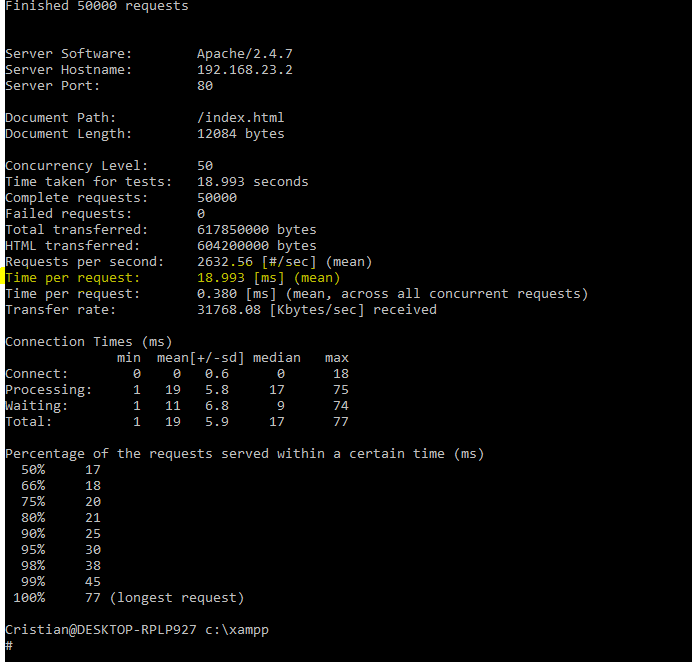
\includegraphics[scale=0.5]{pics/14}  %el parámetro scale permite agrandar o achicar la imagen. En el nombre de archivo puede especificar directorios
		\caption{Configuración modificada} \label{fig:8}
	\end{figure}
	
\end{itemize}

Como podemos apreciar con la configuración personalizada hemos reducido el tiempo medio por petición en 1 ms.

\end{enumerate}



\bibliography{citas} %archivo citas.bib que contiene las entradas 
\bibliographystyle{plain} % hay varias formas de citar

\end{document}
\grid
